\documentclass[journal, a4paper]{IEEEtran}

% some very useful LaTeX packages include:

%\usepackage{cite}      % Written by Donald Arseneau
                        % V1.6 and later of IEEEtran pre-defines the format
                        % of the cite.sty package \cite{} output to follow
                        % that of IEEE. Loading the cite package will
                        % result in citation numbers being automatically
                        % sorted and properly "ranged". i.e.,
                        % [1], [9], [2], [7], [5], [6]
                        % (without using cite.sty)
                        % will become:
                        % [1], [2], [5]--[7], [9] (using cite.sty)
                        % cite.sty's \cite will automatically add leading
                        % space, if needed. Use cite.sty's noadjust option
                        % (cite.sty V3.8 and later) if you want to turn this
                        % off. cite.sty is already installed on most LaTeX
                        % systems. The latest version can be obtained at:
                        % http://www.ctan.org/tex-archive/macros/latex/contrib/supported/cite/

\usepackage{graphicx}   % Written by David Carlisle and Sebastian Rahtz
                        % Required if you want graphics, photos, etc.
                        % graphicx.sty is already installed on most LaTeX
                        % systems. The latest version and documentation can
                        % be obtained at:
                        % http://www.ctan.org/tex-archive/macros/latex/required/graphics/
                        % Another good source of documentation is "Using
                        % Imported Graphics in LaTeX2e" by Keith Reckdahl
                        % which can be found as esplatex.ps and epslatex.pdf
                        % at: http://www.ctan.org/tex-archive/info/

%\usepackage{psfrag}    % Written by Craig Barratt, Michael C. Grant,
                        % and David Carlisle
                        % This package allows you to substitute LaTeX
                        % commands for text in imported EPS graphic files.
                        % In this way, LaTeX symbols can be placed into
                        % graphics that have been generated by other
                        % applications. You must use latex->dvips->ps2pdf
                        % workflow (not direct pdf output from pdflatex) if
                        % you wish to use this capability because it works
                        % via some PostScript tricks. Alternatively, the
                        % graphics could be processed as separate files via
                        % psfrag and dvips, then converted to PDF for
                        % inclusion in the main file which uses pdflatex.
                        % Docs are in "The PSfrag System" by Michael C. Grant
                        % and David Carlisle. There is also some information
                        % about using psfrag in "Using Imported Graphics in
                        % LaTeX2e" by Keith Reckdahl which documents the
                        % graphicx package (see above). The psfrag package
                        % and documentation can be obtained at:
                        % http://www.ctan.org/tex-archive/macros/latex/contrib/supported/psfrag/

\usepackage{subfigure} % Written by Steven Douglas Cochran
                        % This package makes it easy to put subfigures
                        % in your figures. i.e., "figure 1a and 1b"
                        % Docs are in "Using Imported Graphics in LaTeX2e"
                        % by Keith Reckdahl which also documents the graphicx
                        % package (see above). subfigure.sty is already
                        % installed on most LaTeX systems. The latest version
                        % and documentation can be obtained at:
                        % http://www.ctan.org/tex-archive/macros/latex/contrib/supported/subfigure/

\usepackage{url}        % Written by Donald Arseneau
                        % Provides better support for handling and breaking
                        % URLs. url.sty is already installed on most LaTeX
                        % systems. The latest version can be obtained at:
                        % http://www.ctan.org/tex-archive/macros/latex/contrib/other/misc/
                        % Read the url.sty source comments for usage information.

%\usepackage{stfloats}  % Written by Sigitas Tolusis
                        % Gives LaTeX2e the ability to do double column
                        % floats at the bottom of the page as well as the top.
                        % (e.g., "\begin{figure*}[!b]" is not normally
                        % possible in LaTeX2e). This is an invasive package
                        % which rewrites many portions of the LaTeX2e output
                        % routines. It may not work with other packages that
                        % modify the LaTeX2e output routine and/or with other
                        % versions of LaTeX. The latest version and
                        % documentation can be obtained at:
                        % http://www.ctan.org/tex-archive/macros/latex/contrib/supported/sttools/
                        % Documentation is contained in the stfloats.sty
                        % comments as well as in the presfull.pdf file.
                        % Do not use the stfloats baselinefloat ability as
                        % IEEE does not allow \baselineskip to stretch.
                        % Authors submitting work to the IEEE should note
                        % that IEEE rarely uses double column equations and
                        % that authors should try to avoid such use.
                        % Do not be tempted to use the cuted.sty or
                        % midfloat.sty package (by the same author) as IEEE
                        % does not format its papers in such ways.

\usepackage{amsmath}    % From the American Mathematical Society
                        % A popular package that provides many helpful commands
                        % for dealing with mathematics. Note that the AMSmath
                        % package sets \interdisplaylinepenalty to 10000 thus
                        % preventing page breaks from occurring within multiline
                        % equations. Use:
%\interdisplaylinepenalty=2500
                        % after loading amsmath to restore such page breaks
                        % as IEEEtran.cls normally does. amsmath.sty is already
                        % installed on most LaTeX systems. The latest version
                        % and documentation can be obtained at:
                        % http://www.ctan.org/tex-archive/macros/latex/required/amslatex/math/


\usepackage{mathbbol}
\makeatletter
\newif\if@restonecol
\makeatother
\let\algorithm\relax
\let\endalgorithm\relax
\usepackage[linesnumbered,ruled,vlined]{algorithm2e}%[ruled,vlined]{
\usepackage{algpseudocode}
\usepackage{amsmath}
\renewcommand{\algorithmicrequire}{\textbf{Input:}}  % Use Input in the format of Algorithm
\renewcommand{\algorithmicensure}{\textbf{Output:}} % Use Output in the format of Algorithm 
% Other popular packages for formatting tables and equations include:

%\usepackage{array}
% Frank Mittelbach's and David Carlisle's array.sty which improves the
% LaTeX2e array and tabular environments to provide better appearances and
% additional user controls. array.sty is already installed on most systems.
% The latest version and documentation can be obtained at:
% http://www.ctan.org/tex-archive/macros/latex/required/tools/

% V1.6 of IEEEtran contains the IEEEeqnarray family of commands that can
% be used to generate multiline equations as well as matrices, tables, etc.

% Also of notable interest:
% Scott Pakin's eqparbox package for creating (automatically sized) equal
% width boxes. Available:
% http://www.ctan.org/tex-archive/macros/latex/contrib/supported/eqparbox/

% *** Do not adjust lengths that control margins, column widths, etc. ***
% *** Do not use packages that alter fonts (such as pslatex).         ***
% There should be no need to do such things with IEEEtran.cls V1.6 and later.


% Your document starts here!
\begin{document}
\begin{titlepage}

\newcommand{\HRule}{\rule{\linewidth}{0.5mm}} % Defines a new command for the horizontal lines, change thickness here

\center % Center everything on the page
 %----------------------------------------------------------------------------------------
%	LOGO SECTION
%----------------------------------------------------------------------------------------

~\\[1cm]

\includegraphics{SCUT.png}\\[2cm] % Include a department/university logo - this will require the graphicx package

%----------------------------------------------------------------------------------------
%	TITLE SECTION
%----------------------------------------------------------------------------------------

\HRule \\[1cm]
{ \huge \bfseries The Experiment Report of \textit{Machine Learning} }\\[0.6cm] % Title of your document
\HRule \\[2cm]
%----------------------------------------------------------------------------------------
%	HEADING SECTIONS
%----------------------------------------------------------------------------------------


\textsc{\LARGE \textbf{School:} School of Software Engineering}\\[1cm]
\textsc{\LARGE \textbf{Subject:} Software Engineering}\\[2cm] 

 
%----------------------------------------------------------------------------------------
%	AUTHOR SECTION
%----------------------------------------------------------------------------------------

\begin{minipage}{0.4\textwidth}
\begin{flushleft} \large
\emph{Author:}\\
Lizhao Liu % Your name
\end{flushleft}
\end{minipage}
~
\begin{minipage}{0.4\textwidth}
\begin{flushright} \large
\emph{Supervisor:} \\
Mingkui Tan % Supervisor's Name
\end{flushright}
\end{minipage}\\[2cm]
~
\begin{minipage}{0.4\textwidth}
\begin{flushleft} \large
\emph{Student ID:}\\
201730683109
\end{flushleft}
\end{minipage}
~
\begin{minipage}{0.4\textwidth}
\begin{flushright} \large
\emph{Grade:} \\
Undergraduate
\end{flushright}
\end{minipage}\\[2cm]

% If you don't want a supervisor, uncomment the two lines below and remove the section above
%\Large \emph{Author:}\\
%John \textsc{Smith}\\[3cm] % Your name

%----------------------------------------------------------------------------------------
%	DATE SECTION
%----------------------------------------------------------------------------------------

{\large \today}\\[2cm] % Date, change the \today to a set date if you want to be precise

 
%----------------------------------------------------------------------------------------

\vfill % Fill the rest of the page with whitespace

\end{titlepage}

% Define document title and author
	\title{Recommender System Based on Matrix Factorization}
	\maketitle

% Write abstract here
\begin{abstract}
In this report, we solve the Recommendation System problem based on Matrix Factorization (MF). \\
We perform experiments on three aspects: \\
1. Hidden dimension's impact. \\
2. Loss function's impact. \\
3. Regularizer's impact. \\
\end{abstract}

% Each section begins with a \section{title} command
\section{Introduction}
	% \PARstart{}{} creates a tall first letter for this first paragraph
\PARstart{M}{atrix} Factorization is a class of collaborative filtering algorithms used in recommender systems. Matrix factorization algorithms work by decomposing the user-item interaction matrix into the product of two lower dimensionality rectangular matrices Usually, the user-item interaction matrix is very sparse e.g. a lot of zeros or mising values in it. The adavantage of MF is that it transforms a sparse matrix into two lower dimensionality matrices which are regarded as User Embeddings (UE) and Item Embeddings (IE) respectively. MF is wildly used in academic and industry community, which make it very important for us to fully explore it. We will explore it under different settings. 

% Main Part
\section{Methods and Theory}
In this part, we define Matrix Factorization algorithm.
\subsection{Matrix Factorization}
Given a rating matrix $\mathbf{R} \in \mathbb{R}^{m \times n} $, with sparse ratings from m users to n items. MF factorizes $\mathbf{R}$ into $P$ and $Q$, where $P \in \mathbb{R}^{m \times h }$, $Q \in \mathbb{R}^{n \times h}$ and $h$ is the hidden dimension which is a hyper-parameter. In this way, rating matrix can be expressed as $\mathbf{R} = P Q^{T}$.  Usually, $h \ll min(m, n)$. The Space complexity is $O(m*n)$ for $\mathbf{R}$ and $O((m+n)*h)$ for $P$ and $Q$, where $O((m+n)*h) \ll O(m*n)$. So MF can be used for space saving strategy in some scenarios. Beyond that, the factorized $P$ and $Q$ can be used for unseen user-item pair prediction, which is the core of MF.\par


\section{Experiments}
\subsection{Dataset}
We conduct all the experiments on MovieLens-100k dataset, which contains 10,000 comments from 943 users out of 1682 movies. Each comment's form is $(user_{id}, item_{id}, rating)$, where $ rating \in \{1, 2, 3, 4, 5\}$. We randomly split the dataset into three part: 70,000 training examples, 10,000 validation examples and 20,000 test examples. \par

\subsection{Implementation}
We implement the Matrix Factorization using python and mainly rely on the numpy package. The initializer for $P$ and $Q$ is Xavier uniform initializer, which initial matrix $M$, but bounded to interval $[-a*b, a*b]$, where $n$ is $M \in \mathbb{R}^{a\times b}$. We use Adam optimizer with leraning rate 0.001, set batch size to 256 and epoch to 200. We use $MAE$ as evalutation metric. If not sepecifficly stated, we use $h = 10$, $MSE$ as loss function and $l_2~Regularizer$ as regularizer and penalty cofficient 0.1 in regularizer.  

\subsection{Hidden dimension's impact}
In this section, we explore the influence of hidden dimension in MF. We validate the hidden dimension in MF in a range, e.g. 1, 5, 10, 15, 20, 25, 30. \par 
From Fig~\ref{fig:h_mae} we can see that, bigger $h$ tends to have overfitting problem. As presented in Table~\ref{tab:h_mae}, $d = 10$ gets the best performance in validation set. Surprisingly, $h=1$ still get $MAE$ about $0.7522$ in validation set, which is not very far from the best performance e.g. $0.7259$, but $h=1$ can be very time-efficiency and space-saving.  \par
From Fig~\ref{fig:h_tr_losses} and Fig~\ref{fig:h_val_losses} we can see that, bigger $h$ converges faster. \par
\begin{figure}[!hbt]
	% Center the figure.
	\begin{center}
		% Include the eps file, scale it such that it's width equals the column width. You can also put width=8cm for example...
		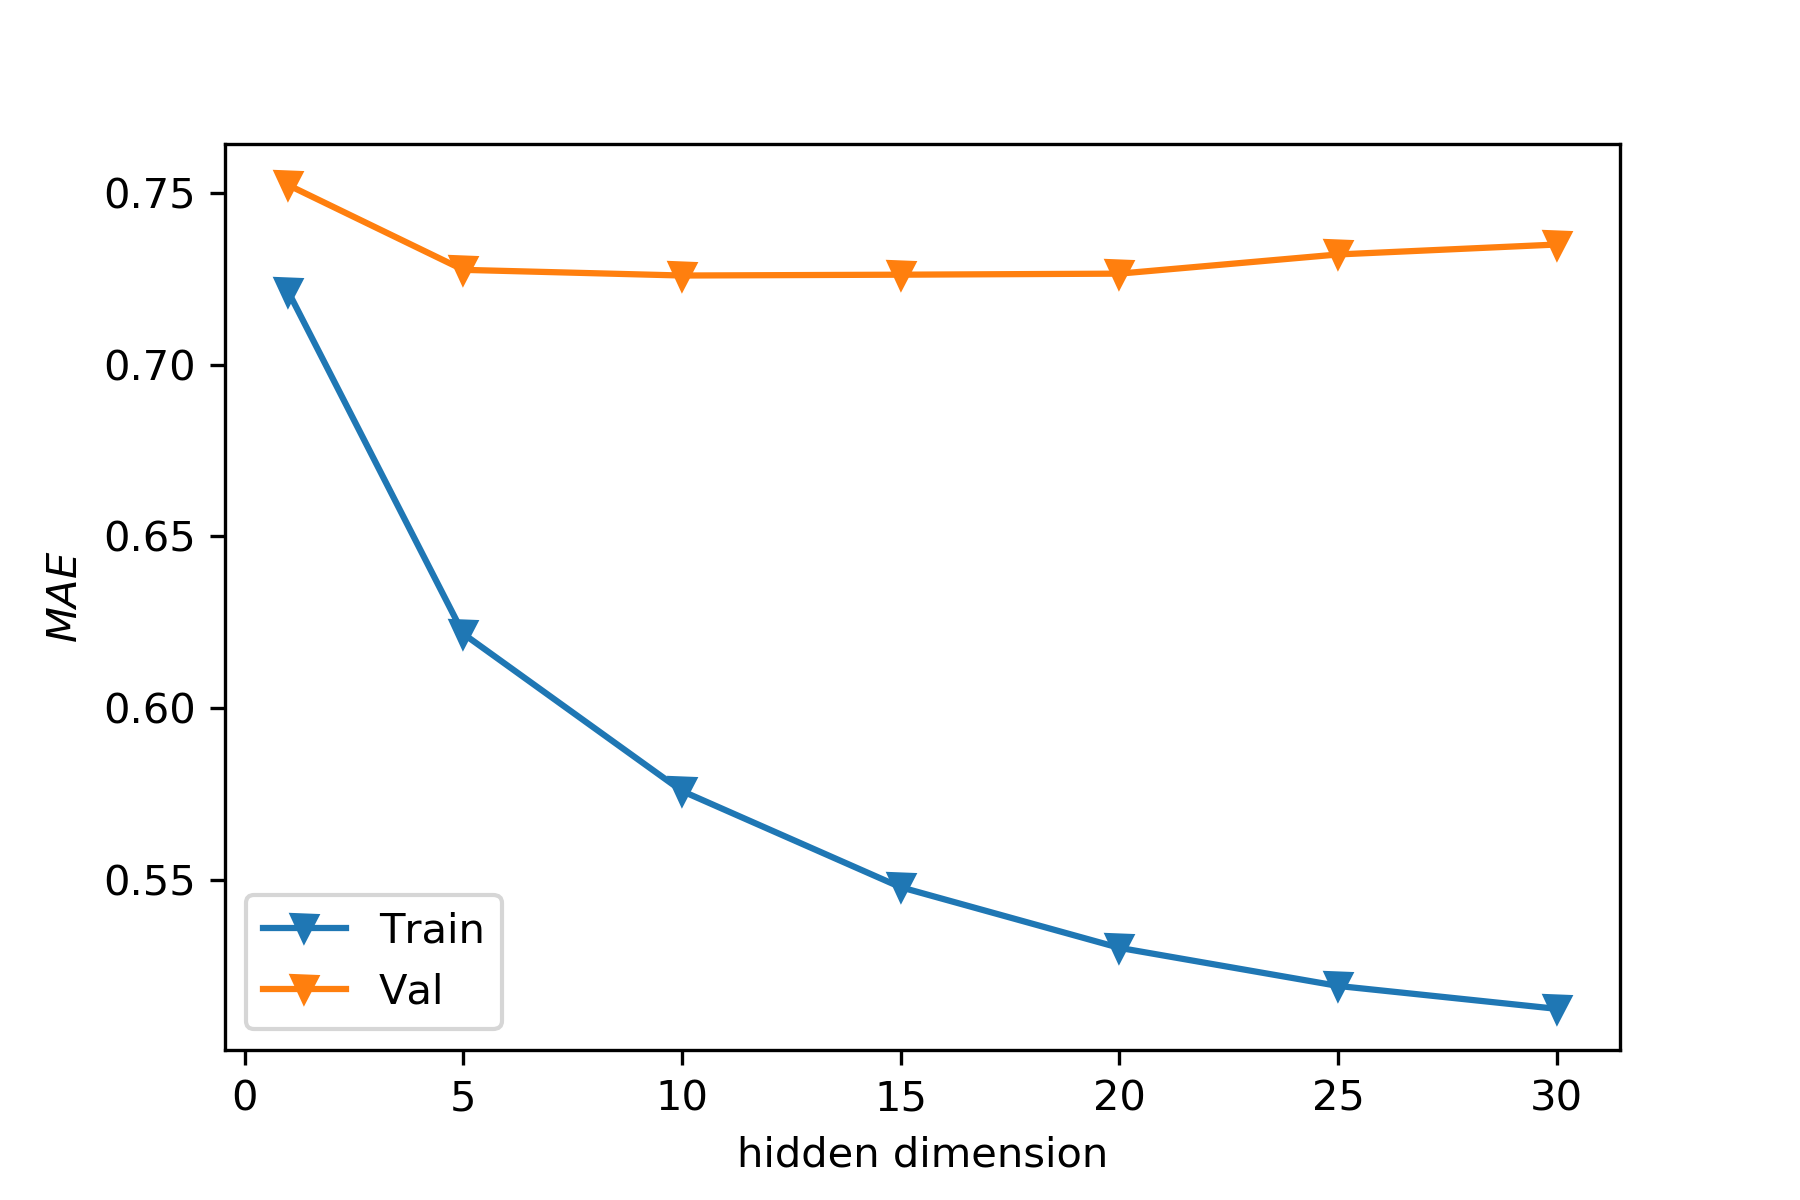
\includegraphics[width=\columnwidth]{h_mae}
		% Create a subtitle for the figure.
		\caption{MF $MAE$ under different $h$.}
		% Define the label of the figure. It's good to use 'fig:title', so you know that the label belongs to a figure.
		\label{fig:h_mae}
	\end{center}
\end{figure} \par

\begin{table}[!hbt]
	% Center the table
	\begin{center}
		% Title of the table
		\caption{MTC $MAE$ under different $h$. Best result are in bold.}
		\label{tab:h_mae}
		% Table itself: here we have two columns which are centered and have lines to the left, right and in the middle: |c|c|
		\begin{tabular}{|c|c|c|c|c|c|c|c|}
			\hline
			$h$  & 1 & 5 & 10 & 15 & 20 & 25 & 30 \\
			\hline
			$MAE_{train}$ & 0.7211 & 0.6216 & 0.5758 & 0.5478 & 0.5302 & 0.5191 & \textbf{0.5124}  \\
			\hline
			$MAE_{val}$  & 0.7522 & 0.7276 & \textbf{0.7259} & 0.7262 & 0.7265 &  0.7321 & 0.7349  \\
			\hline
		\end{tabular}
	\end{center}
\end{table} \par

\begin{figure}[!hbt]
	% Center the figure.
	\begin{center}
		% Include the eps file, scale it such that it's width equals the column width. You can also put width=8cm for example...
		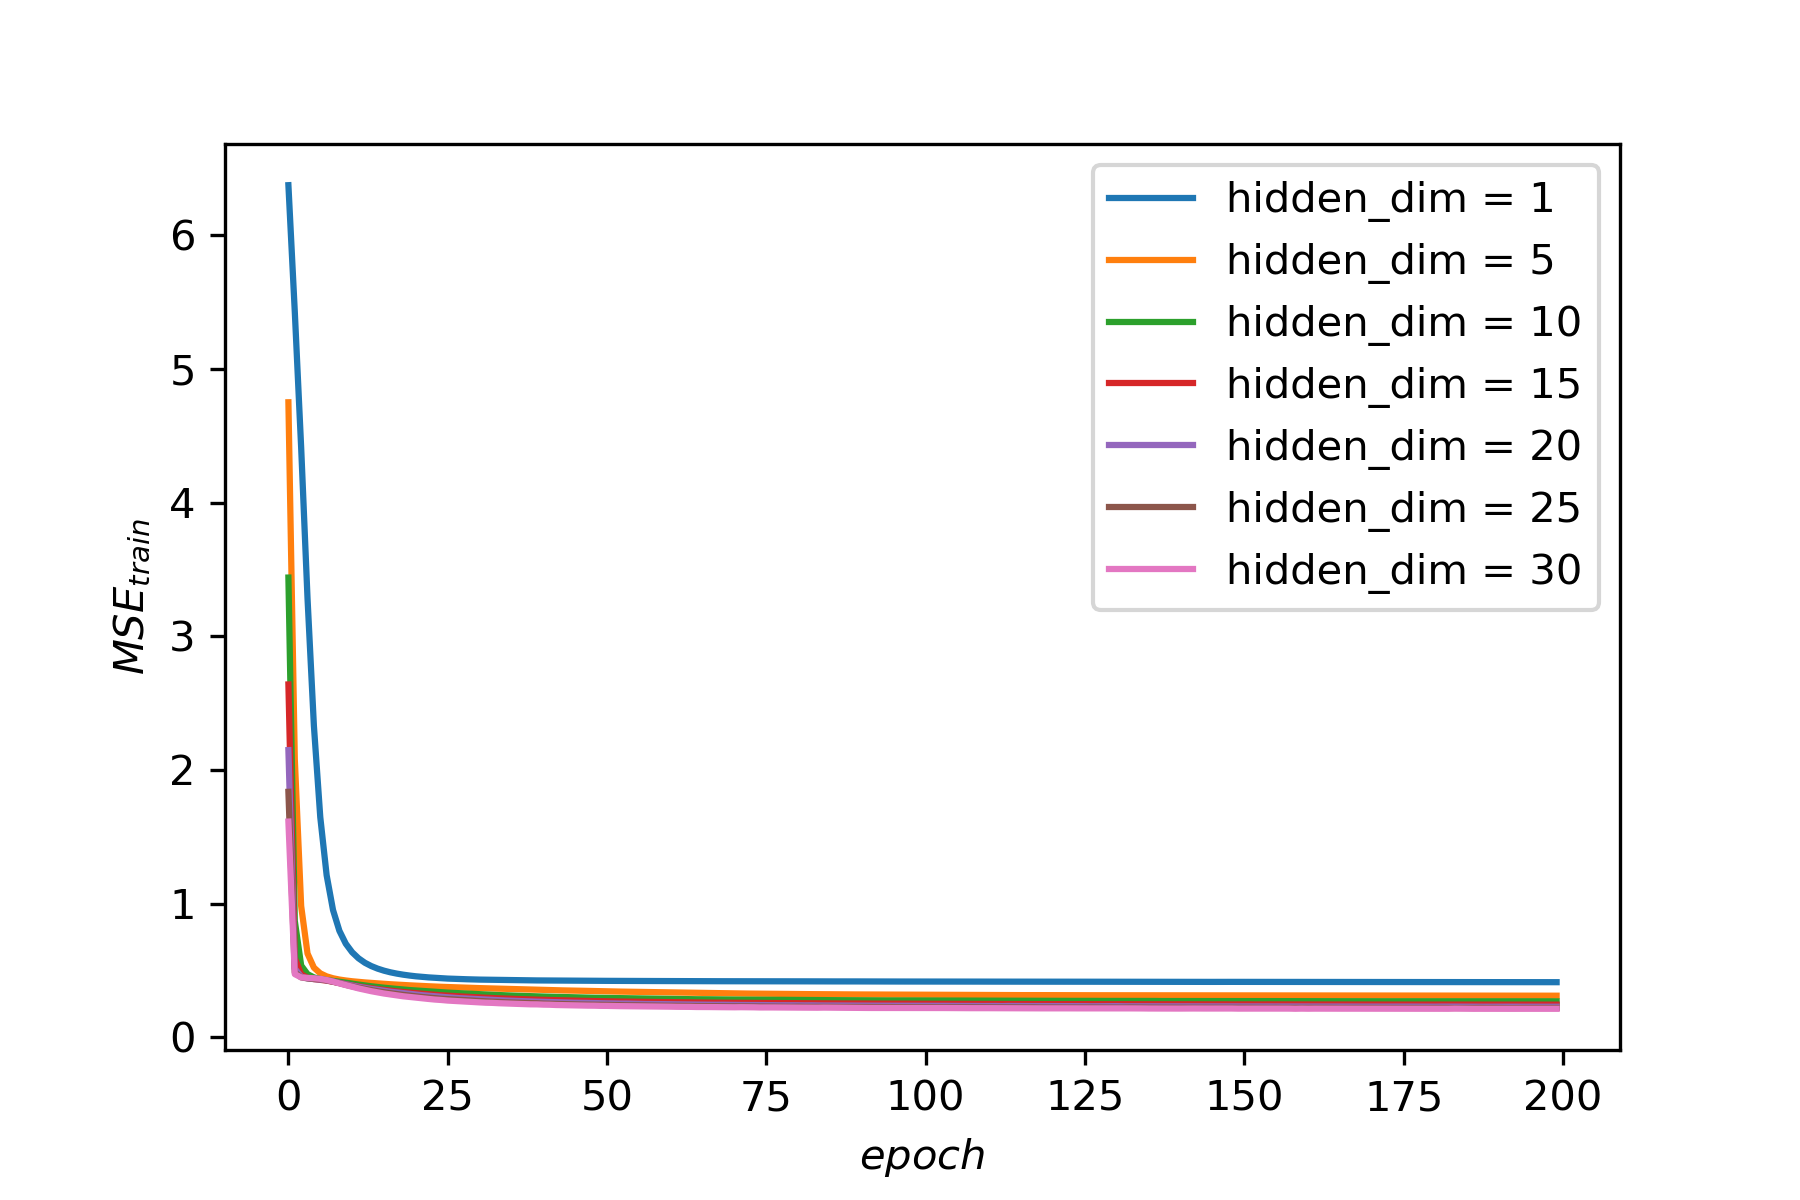
\includegraphics[width=\columnwidth]{h_tr_losses}
		% Create a subtitle for the figure.
		\caption{MF $MSE_{train}$ under different $d$ and $epoch$. }
		% Define the label of the figure. It's good to use 'fig:title', so you know that the label belongs to a figure.
		\label{fig:h_tr_losses}
	\end{center}
\end{figure} \par

\begin{figure}[!hbt]
	% Center the figure.
	\begin{center}
		% Include the eps file, scale it such that it's width equals the column width. You can also put width=8cm for example...
		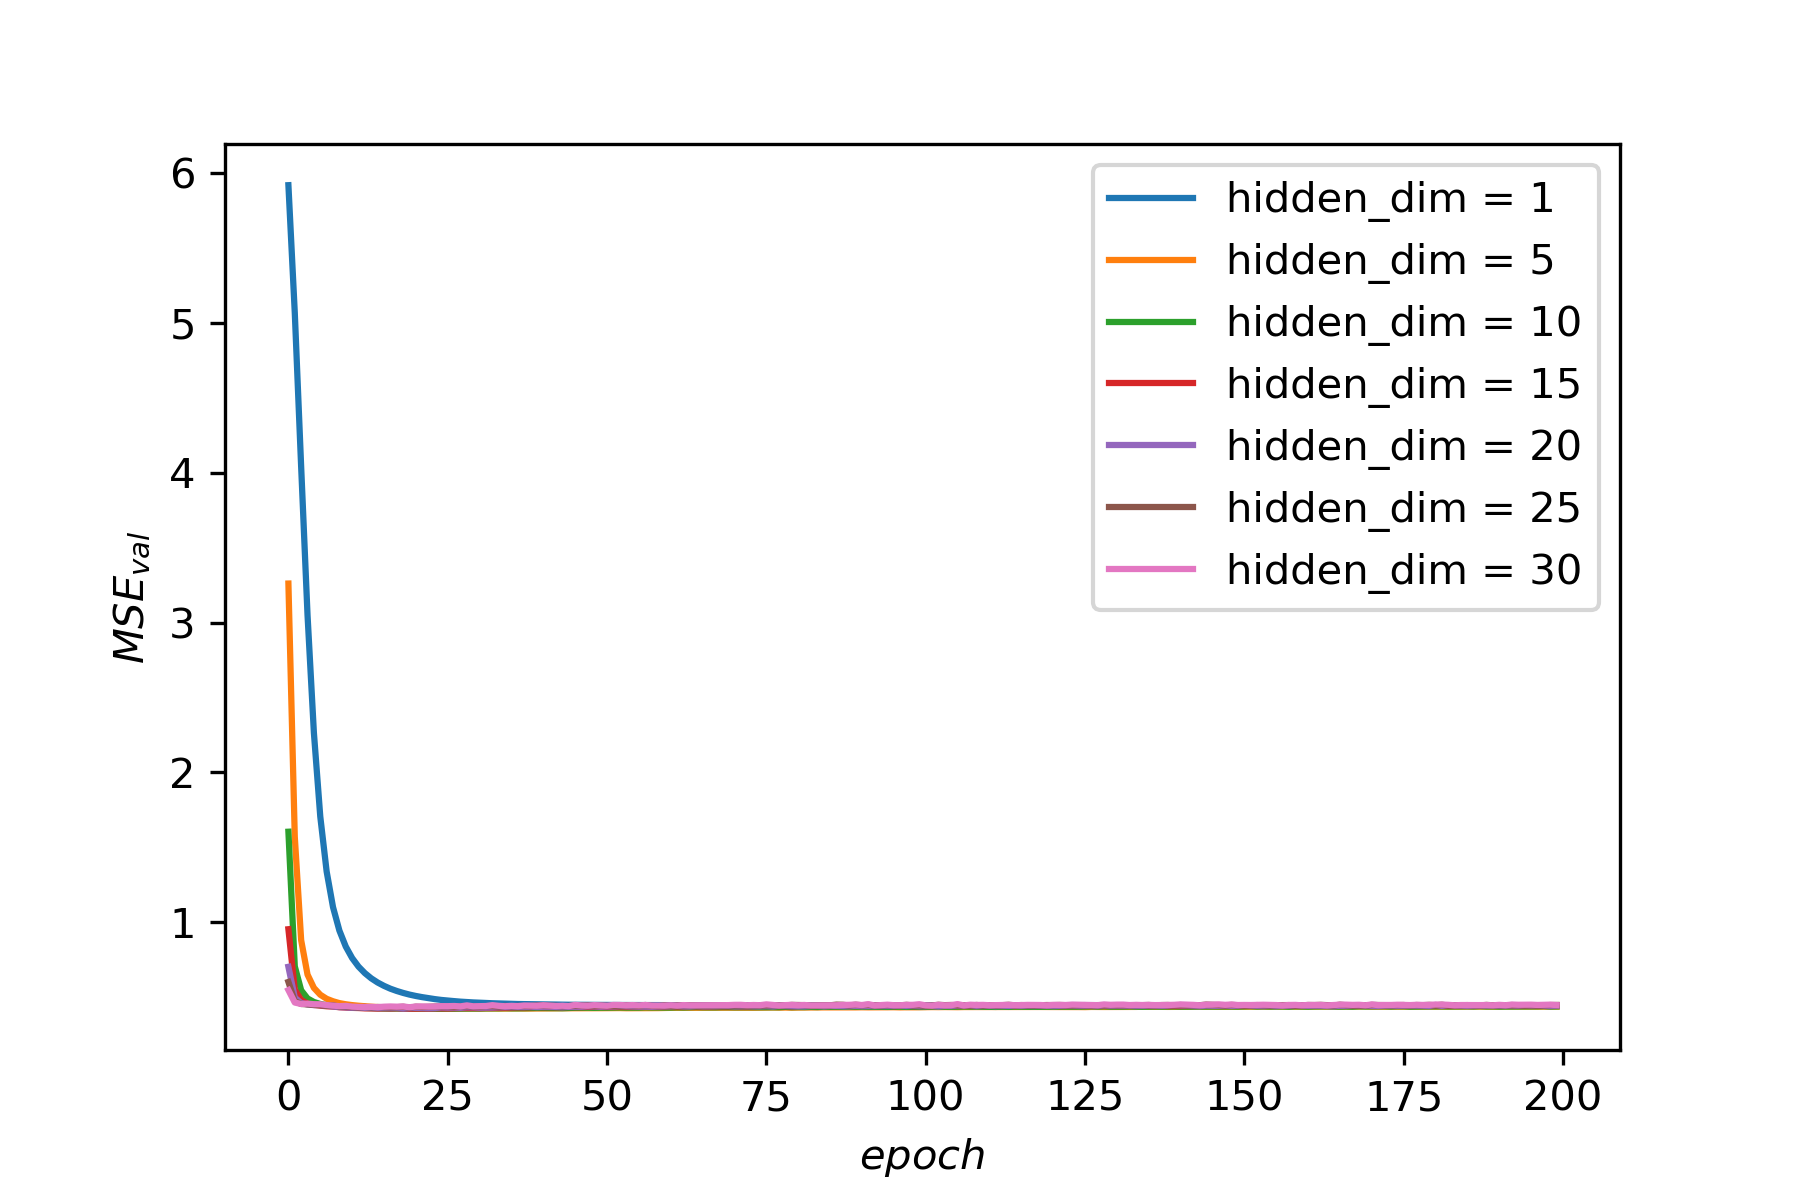
\includegraphics[width=\columnwidth]{h_val_losses}
		% Create a subtitle for the figure.
		\caption{MF $MSE_{val}$ under different $d$ and $epoch$. }
		% Define the label of the figure. It's good to use 'fig:title', so you know that the label belongs to a figure.
		\label{fig:h_val_losses}
	\end{center}
\end{figure} \par



\subsection{Loss function's impact}
In this section, we explore the impact of loss function in MF. In particular, we evaluate three loss functions: \\ \\
1. $MAE(y, \hat{y}) = \frac{1}{m}\Sigma_{i=1}^{m}|y_i - \hat{y_i}|$ \\ \\
2. $MSE(y, \hat{y}) = \frac{1}{2m}\Sigma_{i=1}^{m}(y_i - \hat{y_i})^2$ \\ \\
3. $HB(y, \hat{y}) = \frac{1}{m}\Sigma_{i=1}^{m}L_{\delta }(y_i, \hat{y_i}) $ \\ \\
where, $ L_{\delta }(y_i,\hat{y_i})={\begin{cases}{\frac  {1}{2}}(y_i-\hat{y_i})^{2}&{\textrm  {for}}~|y_i-\hat{y_i}|\leq \delta ,\\\delta \,|y_i-\hat{y_i}|-{\frac  {1}{2}}\delta ^{2}&{\textrm  {otherwise.}}\end{cases}}$ \\ \\
We set $\delta = 1$. \par
Three loss functions are mean absolute error, mean squared error and huber loss respectively. The plot of $MAE(x)$, $MSE(s)$ and $HB(x)$ can be found in Fig~\ref{fig:loss_fns}. Huber Loss can been viewed as a combination of $MSE$ and $MAE$. \par
From Fig~\ref{fig:loss_val_mae}, we can see that, HB gets the best performance on validation set. Intuitively, HB takes MAE's adavantage that robust to outliers and MSE's adavantage that smooth in low error region, so it's prone to perform well. The detailed result can be found in Table~\ref{tab:loss_mae}. \par

\begin{figure}[!hbt]
	% Center the figure.
	\begin{center}
		% Include the eps file, scale it such that it's width equals the column width. You can also put width=8cm for example...
		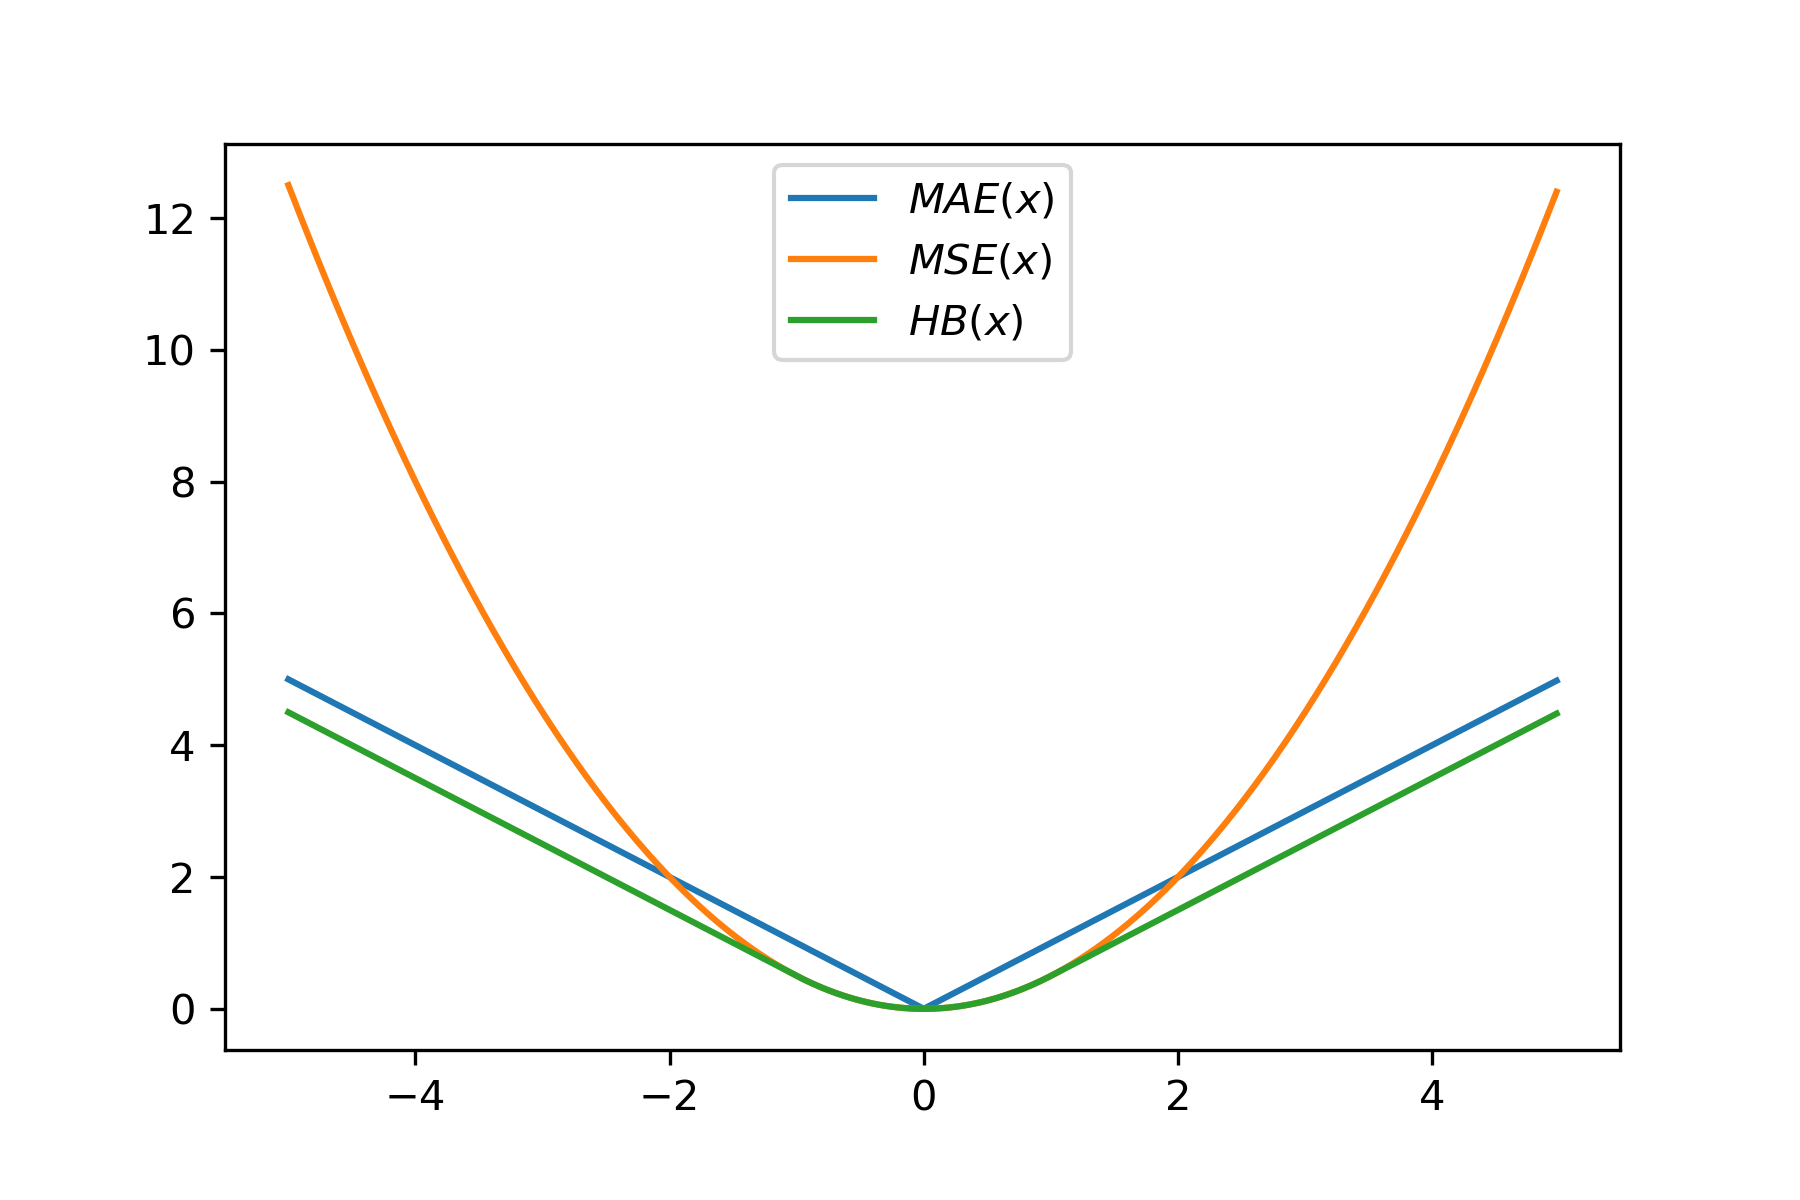
\includegraphics[width=\columnwidth]{loss_fns}
		% Create a subtitle for the figure.
		\caption{$MAE$, $MSE$ and $HB$ plot.}
		% Define the label of the figure. It's good to use 'fig:title', so you know that the label belongs to a figure.
		\label{fig:loss_fns}
	\end{center}
\end{figure} \par

\begin{table}[!hbt]
	% Center the table
	\begin{center}
		% Title of the table
		\caption{MF's performance under different loss function settings. Best result are in bold.}
		\label{tab:loss_mae}
		% Table itself: here we have two columns which are centered and have lines to the left, right and in the middle: |c|c|
		\begin{tabular}{|c|c|c|c|}
			\hline
			$loss_{fn}$  & $MAE$ & $MSE$ & $HB$  \\
			\hline
			$MAE_{val}$ & 0.7293 & 0.7244 & \textbf{0.7217} \\
			\hline
		\end{tabular}
	\end{center}
\end{table} \par

\begin{figure}[!hbt]
	% Center the figure.
	\begin{center}
		% Include the eps file, scale it such that it's width equals the column width. You can also put width=8cm for example...
		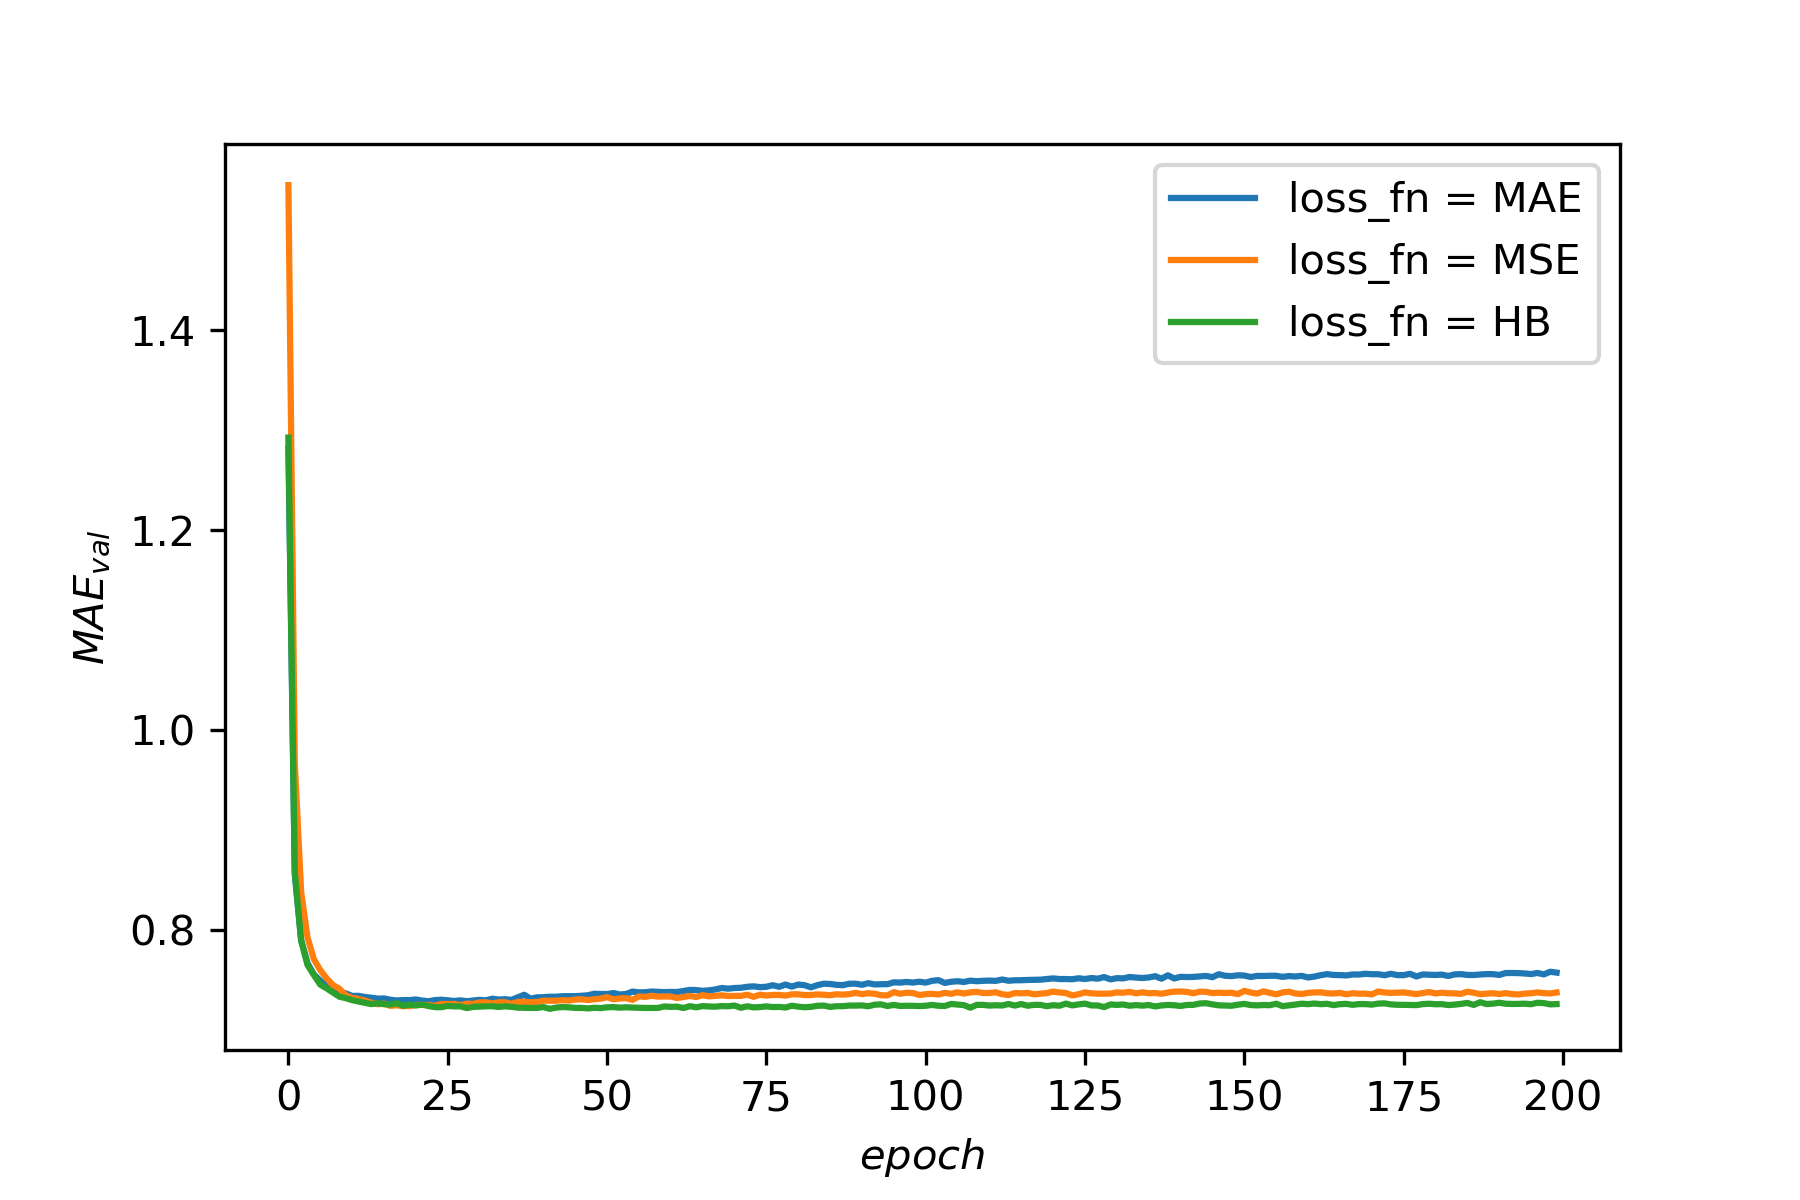
\includegraphics[width=\columnwidth]{loss_val_mae}
		% Create a subtitle for the figure.
		\caption{MF $MAE_{val}$ under different loss functions.}
		% Define the label of the figure. It's good to use 'fig:title', so you know that the label belongs to a figure.
		\label{fig:loss_val_mae}
	\end{center}
\end{figure} \par


\subsection{Regularizer's impact}
In this section, we explore the impact of regularizer in MF. In particular, we evaluate three regularizers: \\ \\
1. $L1(w) = \lambda * \Sigma_{i} |w_i| $ \\ \\
2. $L2(w) = \lambda * \Sigma_{i} w_i^2 $ \\ \\
3. $L1\_L2(w) = \frac{L1(w) + L2(w)}{2}  $ \\ \\
We set $\lambda = 0.01$ in all experiments. \par
$L1\_L2$ regularizer can be seen as a combination of $L1$ and $L2$ regularizer. The plot of three regularizers can be found in Fig~\ref{fig:regs}.\par
From Fig~\ref{fig:reg_val_mae}, we can see that, $L2$ gets the best performance on validation set. $L1\_L2$ has sever overffiting problem than $L1$ and $L2$ after many epoches. However, $L1\_L2$ gets better performance than $L1$.  \par

\begin{figure}[!hbt]
	% Center the figure.
	\begin{center}
		% Include the eps file, scale it such that it's width equals the column width. You can also put width=8cm for example...
		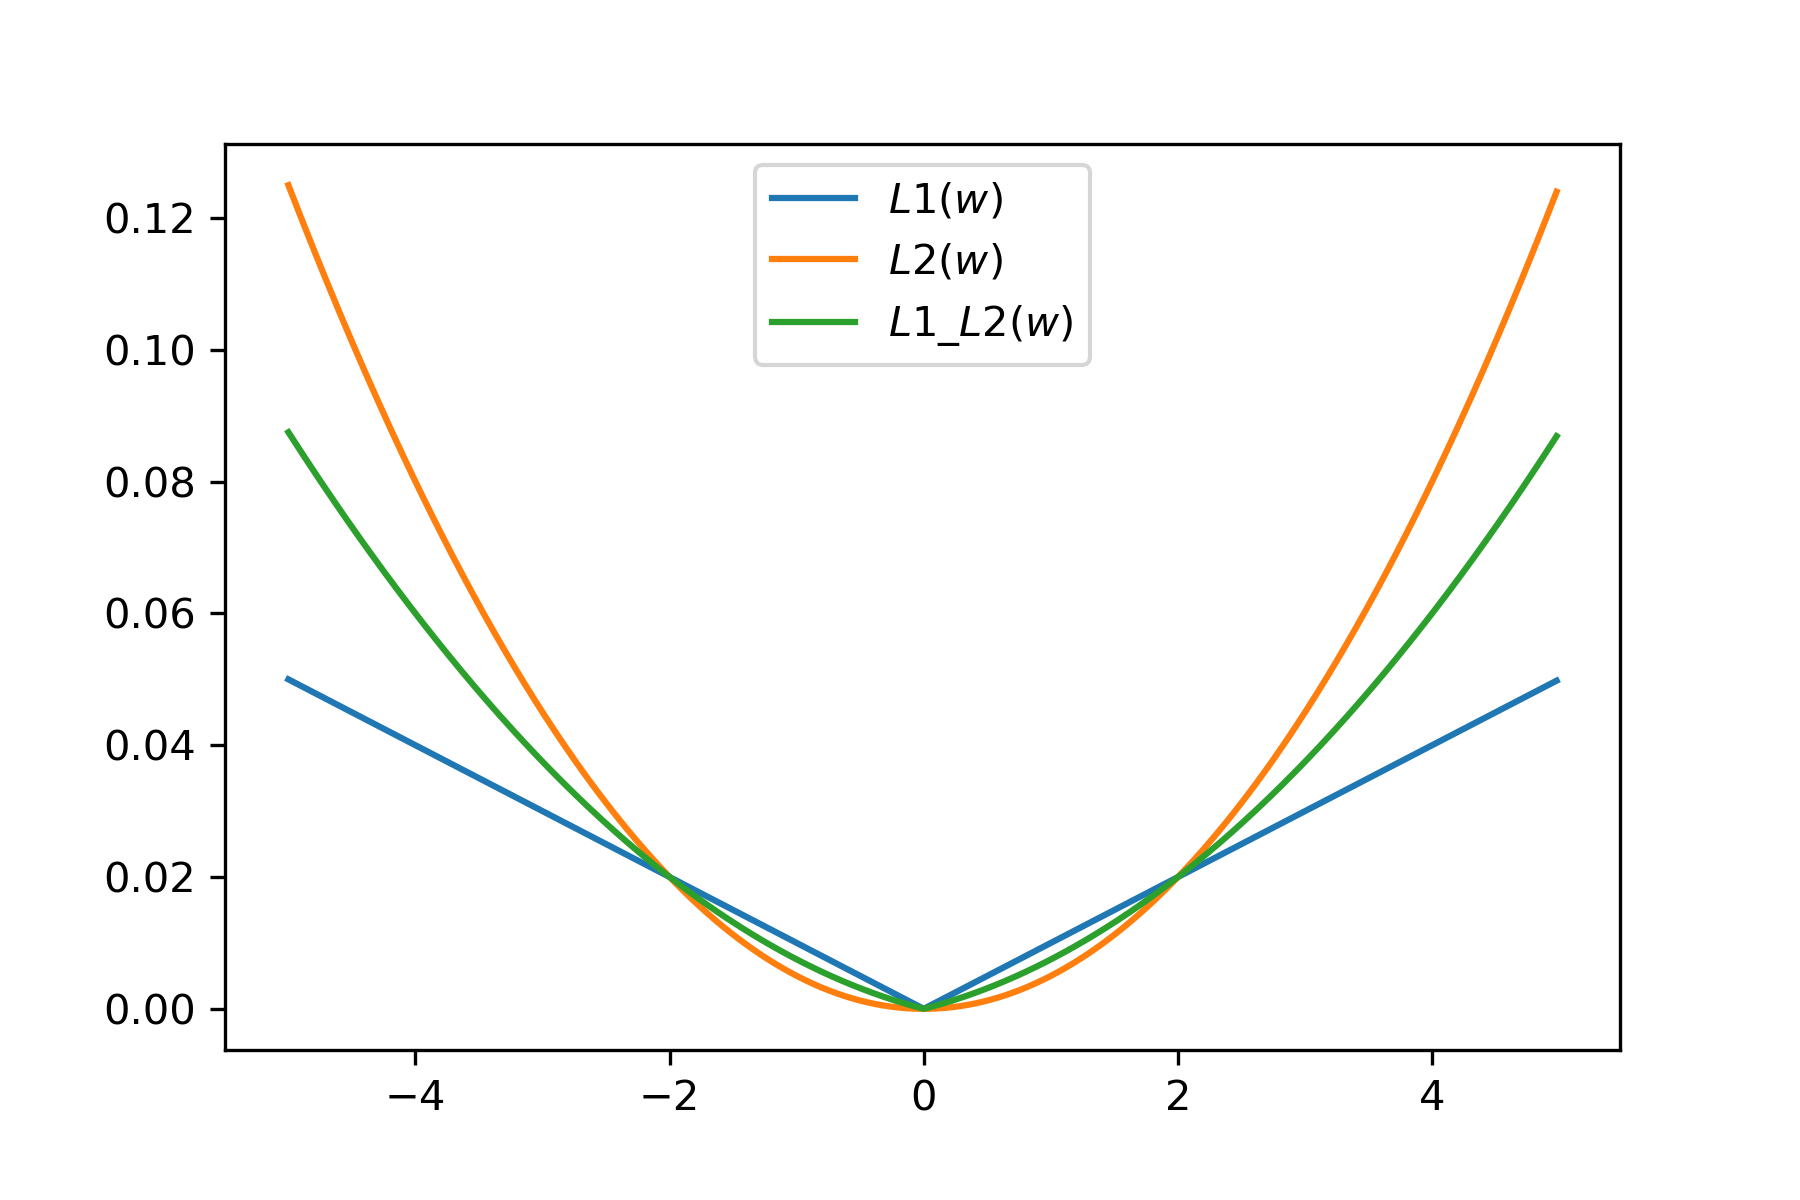
\includegraphics[width=\columnwidth]{regs}
		% Create a subtitle for the figure.
		\caption{$L1$, $L2$ and $L1\_L2$ plot.}
		% Define the label of the figure. It's good to use 'fig:title', so you know that the label belongs to a figure.
		\label{fig:regs}
	\end{center}
\end{figure} \par

\begin{table}[!hbt]
	% Center the table
	\begin{center}
		% Title of the table
		\caption{MF's performance under different regularizer settings. Best result are in bold.}
		\label{tab:reg_mae}
		% Table itself: here we have two columns which are centered and have lines to the left, right and in the middle: |c|c|
		\begin{tabular}{|c|c|c|c|}
			\hline
			$Regularizer$  & $L1$ & $L2$ & $L1\_L2$  \\
			\hline
			$MAE_{val}$ & 0.7537 & \textbf{0.7243} & 0.7358 \\
			\hline
		\end{tabular}
	\end{center}
\end{table} \par

\begin{figure}[!hbt]
	% Center the figure.
	\begin{center}
		% Include the eps file, scale it such that it's width equals the column width. You can also put width=8cm for example...
		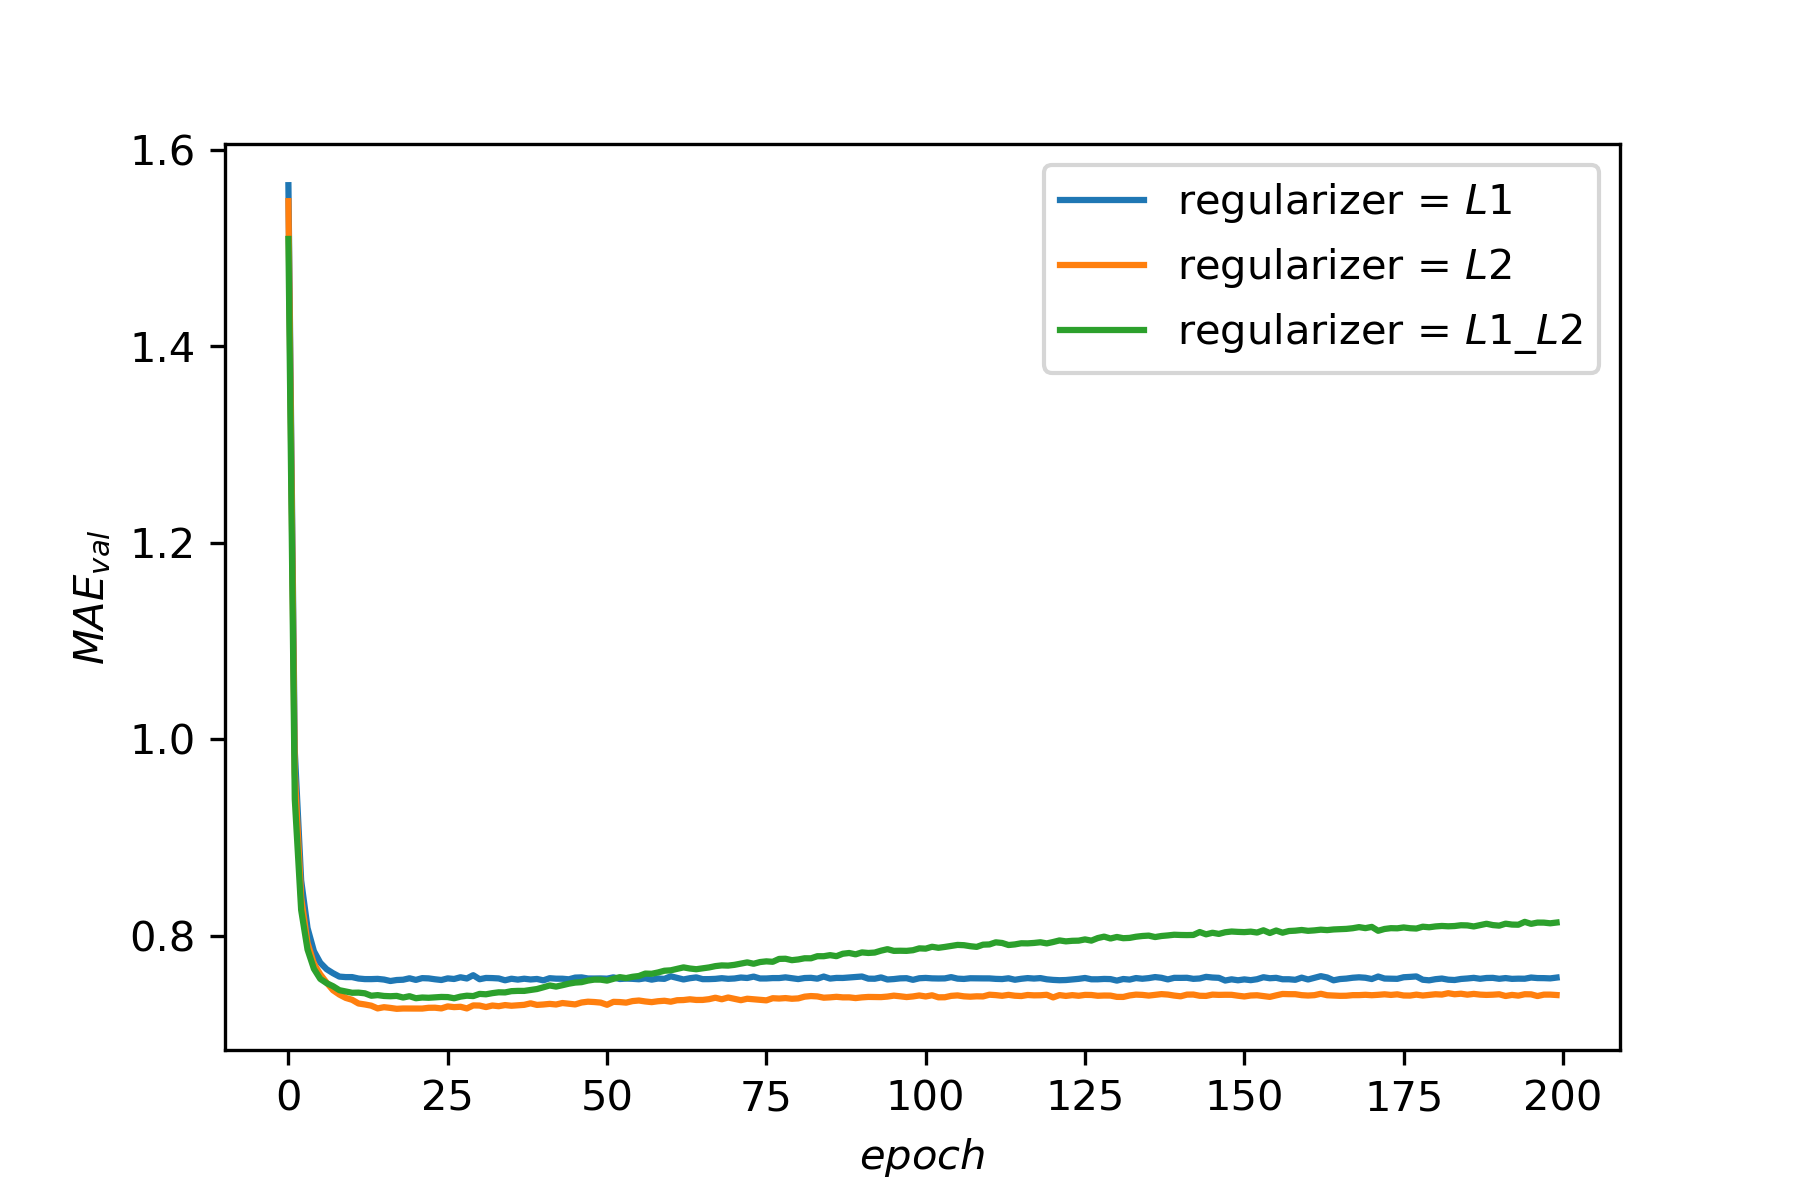
\includegraphics[width=\columnwidth]{reg_val_mae}
		% Create a subtitle for the figure.
		\caption{MF $MAE_{val}$ under different regularizer settings.}
		% Define the label of the figure. It's good to use 'fig:title', so you know that the label belongs to a figure.
		\label{fig:reg_val_mae}
	\end{center}
\end{figure} \par

\subsection{Final Performance}
In this section, we report the final performance under best settings, e.g. $h = 10$, $loss_{fn} = HB$ and $regularizer = L2$. Best result can be found in Table~\ref{tab:final_performance}. \par
\begin{table}[!hbt]
	% Center the table
	\begin{center}
		% Title of the table
		\caption{MF's best performance under best settings.}
		\label{tab:final_performance}
		% Table itself: here we have two columns which are centered and have lines to the left, right and in the middle: |c|c|
		\begin{tabular}{|c|c|c|}
			\hline
			$MAE_{train}$  & $MAE_{val}$ & $MAE_{test}$ \\
			\hline
		      0.6342 & 0.7246 & 0.7294\\
			\hline
		\end{tabular}
	\end{center}
\end{table} \par


\section{Conclusion}
In this report, we explore Matrix Factorization algorithm. Specifically, we explore the hidden dimension $h$, loss function and regularizer in MF. We oberseve that smaller $h$ causes under-fitting problem while bigger $h$ causes over-fitting problem. Under the settings that using Huber Loss as loss function and L2 as regularizer, the best perfomance can be obtained.   \par


% Your document ends here!


\end{document}